In this chapter we introduce the concept of \emph{universality}: eigenvalue statistics of random matrices are largely independent of the distribution of the entries. In particular, we will look at both \emph{global statistics}, i.e., what do histograms of all eigenvalues look like, and \emph{local statistics}, i.e., what do histograms of the largest eigenvalue look like. For the theory we focus on the global statistics (as proving results for the local statistics requires much more sophisticated  mathematical tools), and in particular, we focus on the phenomenon that symmetric matrices with independent, identically distributed (iid) entries have a global statistics that look like the \emph{semicircle}:
\[
{\sqrt{4-x^2} \over 2\ensuremath{\pi}} \qquad \text{for } x \in [-2, 2] \text{ and } 0 \text{ otherwise.}
\]
The \emph{semicircle distribution} can be viewed as a random matrix analogue of  the \emph{normal distribution} $\ensuremath{\scrN}$, whose Probability Density Function (PDF) is a Gaussian:
\[
{\E^{-x^2/2} \over \sqrt{2\ensuremath{\pi}}}.
\]
In this section we will show universality using the \emph{Method of Moments}: we will show that the moments of the statistics converge to the moments of a known distribution. For a scalar random variable $X$ the distribution is generally encoded by the standard moments:
\[
\ensuremath{\bbE} X^k
\]
We will see that in the matrix case the global distribution of eigenvalues is encoded by the matrix-analogue of moments: for $A_n \ensuremath{\in} \ensuremath{\bbR}^{n \ensuremath{\times} n}$ we define
\[
\ensuremath{\bm{\mathrm{E}}} A_n^k := {1 \over n} \ensuremath{\bbE} \Tr A_n^k
\]
where $\Tr$ is the trace of a matrix (sum of the diagonal). 

In particular, we will first discuss the Central Limit Theorem (CLT), a scalar version of universality where the moments of rescaled sums of random variables with finite moments always tend to the moments of a Gaussian. We will then see a similar result for semicircle law, where rescaled matrix moments tend to the moments of a semicircle as the matrix size tends to infinity.

Note that moments are only guaranteed to uniquely define a density in the special case where the probability density decays sufficiently fast, but this is something the Gaussian and semicircle both satisfy.

\textbf{Further reading}: \href{https://terrytao.wordpress.com/wp-content/uploads/2011/02/matrix-book.pdf}{Topics in Random Matrix Theory} by Terry Tao gives a more advanced, higher level introduction to random matrix theory.

\section{Experimental observation of universality}
Before digging into the theory we will do an experimental exploration of universality. Let's begin with the classical Central Limit Theorem (CLT). Consider sampling iid discrete random variables $X_1,\ensuremath{\ldots},X_n$ each taking values $\ensuremath{\pm}1$ with equal probability, so that their expectation is zero and variance is one:
\meeq{
\ensuremath{\bbE} X_k = (-1) {1 \over 2} + 1 {1 \over 2} = 0, \qquad
\ensuremath{\bbE} X_k^2 = (-1)^2 {1 \over 2} + 1^2 {1 \over 2} = 1.
}
By summing and rescaling these variables we can get a new random variable $S_n$:
\[
S_n := {X_1 + \ensuremath{\cdots} + X_n \over \sqrt{n}}.
\]
For large $n$ we can compare a histogram of samples of $S_n$ to a Gaussian:


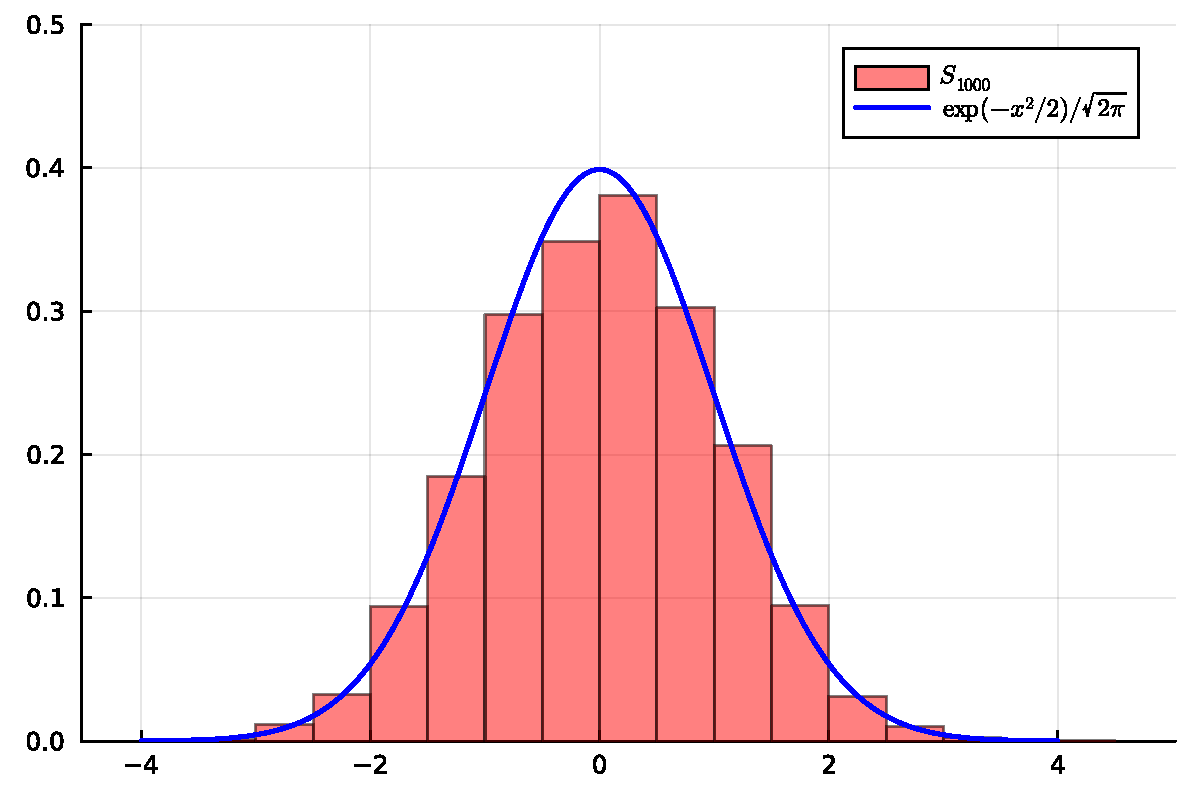
\includegraphics[width=0.6\linewidth,height=0.45\linewidth]{figures/I.Universality_1_1.pdf}

This phenomena is independent of the distribution of $X_k$ provided the moments are finite: we always get a normal distribution (shifted and scaled to match the mean and variance).

We are going to show why this phenomena is true using the Method of Moments: we want to show the moment $\ensuremath{\bbE}[S_n^k]$ tend to the moments of a Gaussian. We can deduce the moments experimentally by averaging over many samples and letting $n$ increase:


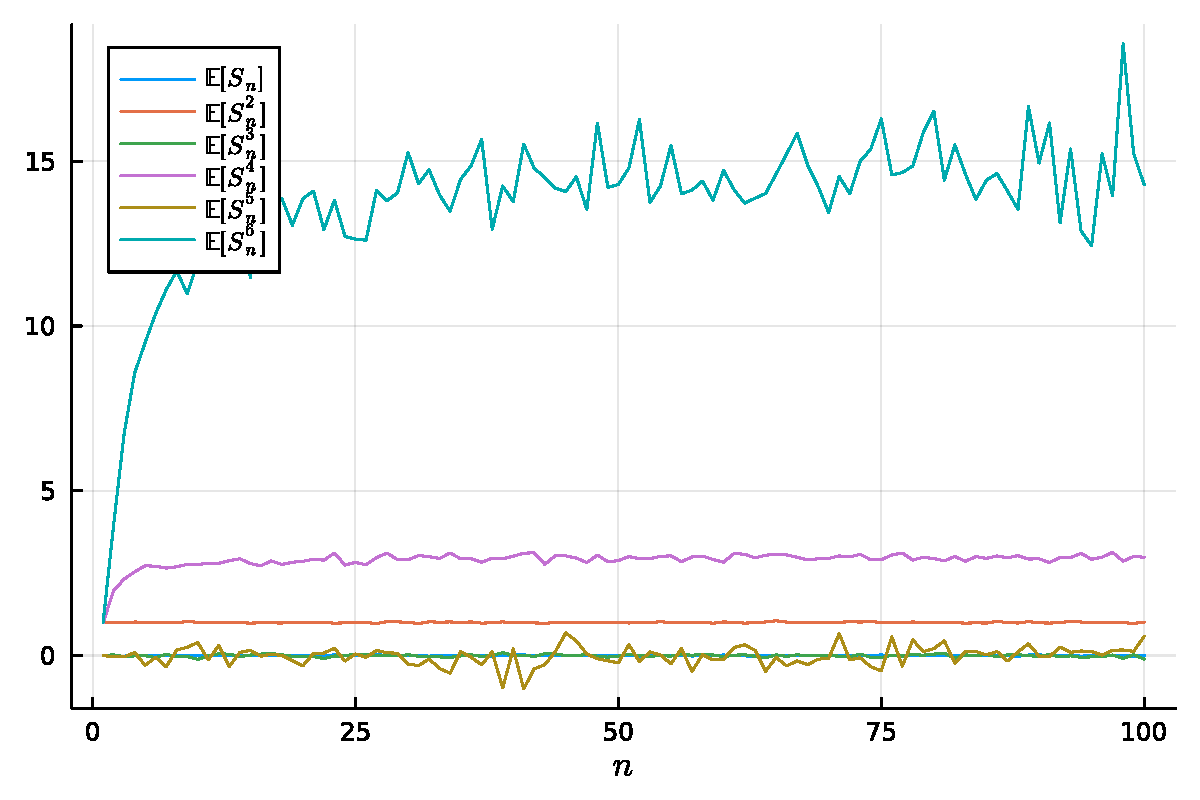
\includegraphics[width=0.6\linewidth,height=0.45\linewidth]{figures/I.Universality_2_1.pdf}

A sensible conjecture then is that $\ensuremath{\bbE}[S_n^k]$ is zero when $k$ is odd and
\[
\ensuremath{\bbE}[S_n^2] \ensuremath{\rightarrow} 1,\quad \ensuremath{\bbE}[S_n^4] \ensuremath{\rightarrow} 3, \quad \ensuremath{\bbE}[S_n^6] \ensuremath{\rightarrow} 15.
\]
Thus we are left with the tasks of: (1) deducing an exact formula for these moments, and (2) proving that the Gaussian has the same moments.

The matrix version of universality involves a histogram of the eigenvalues. Consider $A_n \ensuremath{\in} \ensuremath{\bbR}^{n \ensuremath{\times} n}$ which is symmetric ($A_n = A_n^\ensuremath{\top}$) and whose entries on and above the diagonal are iid random variables taking values $\ensuremath{\pm}1$ with equal probability (and entries below the diagonal defined by symmetry). Each sample of $A_n$ will have $n$ eigenvalues, which we denote $\ensuremath{\sigma}(A_n) = \set{\ensuremath{\lambda}_1,\ensuremath{\ldots},\ensuremath{\lambda}_n}$ (for concreteness we can assume they are sorted from smallest to largest). If we plot a histogram of rescaled eigenvalues $\ensuremath{\sigma}(A_n/ \sqrt{n}) = \set{{\ensuremath{\lambda}_1 \over \sqrt{n}}, \ensuremath{\ldots}, {\ensuremath{\lambda}_n \over \sqrt{n}}}$ of a \emph{single sample} $A_n$ we get a semicircle:


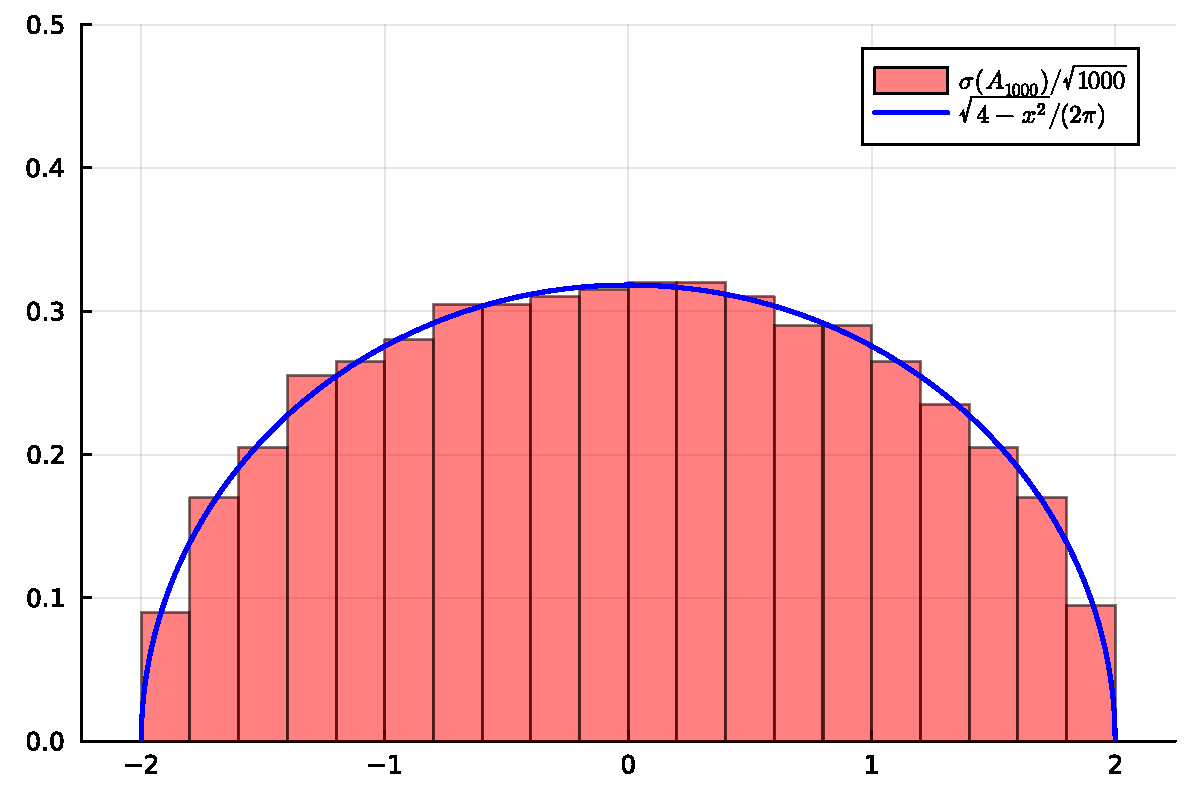
\includegraphics[width=0.6\linewidth,height=0.45\linewidth]{figures/I.Universality_3_1.pdf}

Just as in the CLT, this phenomena is independent of the distribution of the entries of $A_n$ provided the moments are finite: we always get a semicircle (shifted and scaled to match the mean and variance).

Like the CLT we will show this observation using the Method of Moments, and again we can deduce the moments experimentally by letting $n$ increase (a single sample per $n$ works in this case):


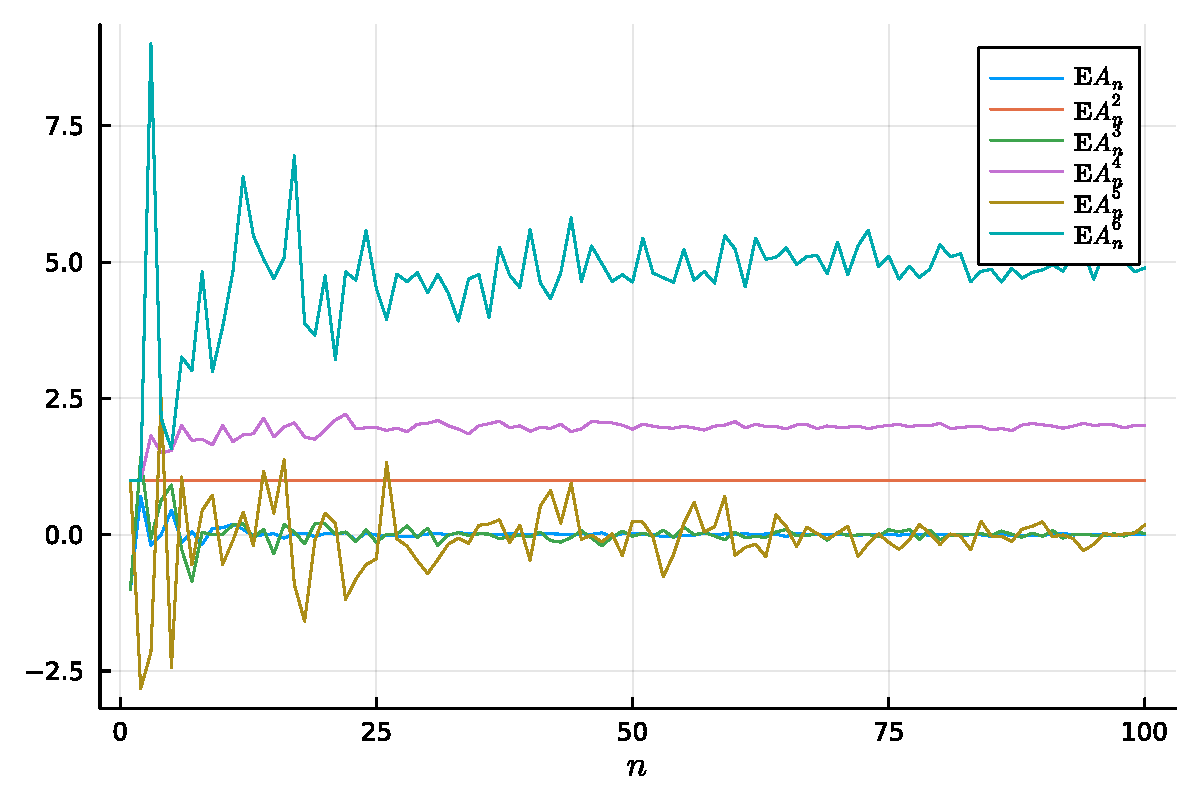
\includegraphics[width=0.6\linewidth,height=0.45\linewidth]{figures/I.Universality_4_1.pdf}

Again the odd moments appear to be zero but now we might conjecture that the even moments satisfy
\[
\ensuremath{\bm{\mathrm{E}}}A_n^2 \ensuremath{\rightarrow} 1,\quad \ensuremath{\bm{\mathrm{E}}}A_n^4 \ensuremath{\rightarrow} 2,\quad \ensuremath{\bm{\mathrm{E}}}A_n^6 \ensuremath{\rightarrow} 5.
\]
Again we are left with the tasks of: (1) deducing an exact formula for these moments, and (2) proving that the semicircle has the same moments.

In the remainder of this chapter we sketch out a proof of both the CLT and the semicircle law for random matrices.

\section{Moments of the normal distribution}
We will use the method of moments, so our first step is to establish an explicit formula for the moments of a Gaussian. We will think of this in terms the following combinatorial object:

\begin{definition}[double factorial]
\[
(2m-1)!! := {(2m)! \over 2^m m!} = 1 \ensuremath{\cdot} 3 \ensuremath{\cdot} 5 \ensuremath{\cdots} (2m-1).
\]
\end{definition}

Note this satisfies a simple recurrence:
\[
(2m-1)!! = (2m-1) \ensuremath{\cdot} (2m-3)!! \quad \hbox{for} \quad m > 1.
\]
We can check the first few double factorials:
\[
1!! = 1,\quad 3!! = 3,\quad 4!! = 15
\]
which exactly match our predicted values for the even moments $\ensuremath{\bbE}[S_n^k]$. 

To prove this result we will use a combinatorial argument. Note that the double factorial  counts the number of ways to partition $\{1,\ensuremath{\ldots},2m\}$ into $m$ different pairs, that is to write
\[
\{1,\ensuremath{\ldots},2m\} = \{x_1,y_1\} \ensuremath{\cup} \ensuremath{\cdots} \ensuremath{\cup} \{x_m,y_m\}
\]
where $x_1,\ensuremath{\ldots},x_m,y_1,\ensuremath{\ldots},y_m$ is a permutation of $1,\ensuremath{\ldots},2m$ and $x_k < y_k$ for all $k$. For example, if $m = 2$ then we have the following pairings of $1,2,3,4$:
\[
\{1,2\}, \{3,4\} \qquad \{1,3\}, \{2,4\} \qquad \{1,4\}, \{2,3\}
\]
and thus $3!! = 3$. And if $m = 3$ then we have $5!! = 15$ total pairings:
\begin{align*}
\{1,2\}, \{3,4\}, \{5,6\} &\qquad \{1,2\}, \{3,5\}, \{4,6\} \qquad \{1,2\}, \{3,6\}, \{4,5\} \\
\{1,3\}, \{2,4\}, \{5,6\} &\qquad \{1,3\}, \{2,5\}, \{4,6\} \qquad \{1,3\}, \{2,6\}, \{4,5\} \\
\{1,4\}, \{2,3\}, \{5,6\} &\qquad \{1,4\}, \{2,5\}, \{3,6\} \qquad \{1,4\}, \{2,6\}, \{3,5\} \\
\{1,5\}, \{2,3\}, \{4,6\} &\qquad \{1,5\}, \{2,4\}, \{3,6\} \qquad \{1,5\}, \{2,6\}, \{3,4\} \\
\{1,6\}, \{2,3\}, \{4,5\} &\qquad \{1,6\}, \{2,4\}, \{3,5\} \qquad \{1,6\}, \{2,5\}, \{3,4\}.
\end{align*}
This can be deduced by a very simple inductive argument. When $m = 1$ we have exactly $1!! = 1$ pairings. For $m > 1$,  assuming the number of pairings for $n < m$ is given by $(2n-1)!!$. We can pair $1$ with a choice of the $2m-1$ numbers: $2,3,\ensuremath{\ldots},$ or $2m$. But then by the induction hypothesis the remaining $2m-2$ numbers have exactly $(2m-3)!!$ pairings. Thus we have
\[
(2m-1)!! = (2m-1) \cdot (2m-3)!!
\]
which exactly matches the simple recurrence formula.

We now show the moments of a Gaussian are given in terms of the double factorial:

\begin{lemma}[Gaussian moments]
\[
\ensuremath{\mu}_k := \ensuremath{\int}_{-\ensuremath{\infty}}^\ensuremath{\infty} x^k {\E^{-x^2/2}  \over \sqrt{2\ensuremath{\pi}}} \dx = \begin{cases}
0 & \hbox{\textrm{if  $k$ is odd}} \\
{(k-1)!!} & \hbox{\textrm{if $k$ is even}}
\end{cases}
\]
\end{lemma}
\textbf{Proof} 

We begin with a more formal explanation.  The case of $k$ odd follows from symmetry. For even $k$ we  use a proof by induction. The base case of $k = 0$ follows using the classic trick of computing the integral of a Gaussian by turning it into a 2D integral, using polar coordinates ($r^2 = x^2 + y^2$) and the change of variables $t = r^2/2$:
\meeq{
\pr(\ensuremath{\int}_{-\ensuremath{\infty}}^\ensuremath{\infty} \E^{-x^2/2} \dx)^2 = \pr(\ensuremath{\int}_{-\ensuremath{\infty}}^\ensuremath{\infty} \E^{-x^2/2} \dx)\pr(\ensuremath{\int}_{-\ensuremath{\infty}}^\ensuremath{\infty} \E^{-y^2/2} \dy) =
\ensuremath{\int}_{-\ensuremath{\infty}}^\ensuremath{\infty} \ensuremath{\int}_{-\ensuremath{\infty}}^\ensuremath{\infty} \E^{-(x^2+y^2)/2} \dx \dy \ccr
= \ensuremath{\int}_0^\ensuremath{\infty} \ensuremath{\int}_0^{2\ensuremath{\pi}}  r \E^{-r^2/2} \dr \D\ensuremath{\theta}  = 2\ensuremath{\pi} \ensuremath{\int}_0^\ensuremath{\infty}  \E^{-t} \dt =2\ensuremath{\pi},
}
hence
\[
\ensuremath{\mu}_0 = {\ensuremath{\int}_{-\ensuremath{\infty}}^\ensuremath{\infty} \E^{-x^2/2} \dx \over \sqrt{2\ensuremath{\pi}}} = 1.
\]
For even $k> 0$ assume it is true for all smaller $k$. Then we can integrate-by-parts to deduce:
\meeq{
\sqrt{2\ensuremath{\pi}} \ensuremath{\mu}_k = \ensuremath{\int}_{-\ensuremath{\infty}}^\ensuremath{\infty} x^k \E^{-x^2/2} \dx = \ensuremath{\int}_{-\ensuremath{\infty}}^\ensuremath{\infty} x^{k-1} \underbrace{x \E^{-x^2/2}}_{=-{\D \over \dx}  \E^{-x^2/2}} \dx \ccr
= [-x^{k-1} \E^{-x^2/2}]_{-\ensuremath{\infty}}^\ensuremath{\infty} + (k-1) \ensuremath{\int}_{-\ensuremath{\infty}}^\ensuremath{\infty} x^{k-2} \E^{-x^2/2} \dx =  \sqrt{2\ensuremath{\pi}} (k-1) \ensuremath{\mu}_{k-2}.
}
I.e., $\ensuremath{\mu}_k = (k-1) \ensuremath{\mu}_{k-2}$, but this is exactly the formula that we showed $(k-1)!!$ satisfies above (if we write $k = 2m$).

\ensuremath{\QED}

\section{Central Limit Theorem}
We now want to show that the moments $\ensuremath{\bbE}[S_n^k]$ for
\[
S_n := {X_1 + \ensuremath{\ldots} + X_n \over \sqrt{n}}.
\]
match those of the Gaussian, and hence are also given by the double factorial as $n \ensuremath{\rightarrow} \ensuremath{\infty}$. This implicitly tells us that the distribution converges to a Gaussian.  We will use the \emph{multinomial theorem}:

\begin{theorem}[multinomial theorem] 
\[
(X_1 + \ensuremath{\cdots} + X_n)^k = \ensuremath{\sum}_{k_1 + \ensuremath{\cdots} + k_n = k}  {k! \over k_1! \ensuremath{\cdots} k_n!} X_1^{k_1} \ensuremath{\cdots} X_n^{k_n}.
\]
\end{theorem}
\textbf{Proof} This is a generalisation of the binomial theorem, and can be proved by induction on $k$. The base case of $n = 1$ is trivial and the case $n = 2$ is equivalent to the binomial theorem. For $n \ensuremath{\geq} 2$ we write:
\begin{align*}
(X_1 + \ensuremath{\cdots} +& X_{n-1} + X_n + X_{n+1})^k = (X_1 + \ensuremath{\cdots} + X_{n-1} + (X_n + X_{n+1}))^k \ccr 
= \ensuremath{\sum}_{k_1 + \ensuremath{\cdots} + k_{n-1} + \ensuremath{\kappa} = k}  {k! \over k_1! \ensuremath{\cdots} k_{n-1}! \ensuremath{\kappa}!} X_1^{k_1} \ensuremath{\cdots} X_{n-2}^{k_{n-2}} (X_n + X_{n+1})^\ensuremath{\kappa} \ccr
= \ensuremath{\sum}_{k_1 + \ensuremath{\cdots} + k_{n-1} + \ensuremath{\kappa} = k}  {k! \over k_1! \ensuremath{\cdots} k_{n-1}!\ensuremath{\kappa}!} X_1^{k_1} \ensuremath{\cdots} X_{n-2}^{k_{n-2}} \ensuremath{\sum}_{k_n + k_{n+1} = \ensuremath{\kappa}}  {\ensuremath{\kappa}! \over k_n! k_{n+1}!} X_n^{k_n} X_{n+1}^{k_{n+1}}
\end{align*}
where we have used the binomial theorem in the last step. But we now note we can combine the two sums as a single sum to deduce:
\begin{align*}
(X_1 + \ensuremath{\cdots} +& X_{n-1} + X_n + X_{n+1})^k = 
\ensuremath{\sum}_{k_1 + \ensuremath{\cdots} + k_{n+1} = k}  {k! \over k_1! \ensuremath{\cdots} k_{n-1}!\ensuremath{\kappa}!}  {\ensuremath{\kappa}! \over k_n! k_{n+1}!}   X_1^{k_1} \ensuremath{\cdots} X_{n+1}^{k_{n+1}} \ccr
= \ensuremath{\sum}_{k_1 + \ensuremath{\cdots} + k_{n+1} = k}  {k! \over k_1! \ensuremath{\cdots} k_{n-1}!k_n!k_{n+1}!}     X_1^{k_1} \ensuremath{\cdots} X_{n+1}^{k_{n+1}}.
\end{align*}
\ensuremath{\QED}

This basic result allows us to exapnd out the moments and deduce the main result:

\begin{theorem}[CLT] Let $X_1, X_2, \ensuremath{\ldots}$ be iid variables with $\ensuremath{\bbE}[X_j] = 0$, $\ensuremath{\bbE}[X_j^2] = 1$, and all other moments are finite. Then for all $k$ we have
\[
\ensuremath{\bbE}[S_n^k] \underset{n \ensuremath{\rightarrow} \ensuremath{\infty}}{\ensuremath{\longrightarrow}} \ensuremath{\mu}_k.
\]
\end{theorem}
\textbf{Proof}

We have from the multinomial theorem and independence:
\[
\ensuremath{\bbE}[S_n^k] = n^{-k/2} \ensuremath{\sum}_{k_1 + \ensuremath{\cdots} + k_n = k}  {k! \over k_1! \ensuremath{\cdots} k_n!}  \ensuremath{\bbE}[X_1^{k_1}] \ensuremath{\cdots}  \ensuremath{\bbE}[X_n^{k_n}].
\]
We claim when $k = 2m$ that the sum is dominated by the terms where the $k_j$ are either zero or 2, in particular, where there are precisely $m$ 2s. In particular, we have to choose $m$ indices to have $k_j = 2$ from a total of $n$, and  there are exactly
\[
\begin{pmatrix} n \\ m \end{pmatrix} = {n! \over m! (n-m)!}
\]
of these. Noting that $\ensuremath{\bbE}[X_k^2] = \ensuremath{\bbE}[X_k^0]$,  these terms each take a value of
\[
n^{-m} {(2m)! \over 2^m}  \ensuremath{\bbE}[X_1^{k_1}] \ensuremath{\cdots}  \ensuremath{\bbE}[X_n^{k_n}] = {(2m)! \over (2n)^m},
\]
giving a total contribution of
\[
{n! (2m)! \over (2n)^m m! (n-m)!}  \ensuremath{\rightarrow} {(2m)! \over 2^m m!}  = (2m-1)!!
\]
where we use the fact that, for $m$ fixed,
\[
{n! \over (n-m)! n^m} = {n (n-1) \ensuremath{\cdots} (n-m+1) \over n^m} = {n^m + O(n^{m-1}) \over n^m} \ensuremath{\rightarrow} 1
\]
as $n \ensuremath{\rightarrow} \ensuremath{\infty}$.

We are just left with showing the total contribution from all other choices of $k_1 + \ensuremath{\cdots} + k_n = k$ tend to zero. Note that the terms where any $k_j = 1$ contribute zero as $\ensuremath{\bbE}[X_j] = 0$. Showing the remaining terms don't contribute as $n \ensuremath{\rightarrow} \ensuremath{\infty}$ (and that in the odd case no terms contribute) is a bit technical so we omit the details.

\ensuremath{\QED}

\textbf{Remark} Note the assumption of finite moments is essential. A classic counter example is if $X_k$ have a heavy-tail distribution like the Cauchy distribution:
\[
{1 \over \ensuremath{\pi}} {1 \over x^2 + 1}.
\]
Not even the first moment exists, that is, this distribution has no mean! (Symmetry may make one think that the mean should be zero, but if we average samples it never converges.) If we take iid samples $X_k$ of the Cauchy distribution we know that
\[
{X_1 + \ensuremath{\cdots} + X_n \over n}
\]
is the same Cauchy distribution. (Note the division by $n$, not $\sqrt{n}$, which differs from the CLT above.)

\section{Wigner ensembles and global statistics}
To discuss universality in the setting of random matrices we focus on symmetric matrices with iid entries, i.e., the \emph{Wigner ensembles}:

\begin{definition}[Wigner] A random matrix $A_n \ensuremath{\in} \ensuremath{\bbR}^{n \ensuremath{\times} n}$ is a Wigner matrix if:

\begin{itemize}
\item[1. ] The entries $a_{kj}$ for $j \ensuremath{\geq} k$ are all iid with mean 0, variance 1, and all moments are finite.


\item[2. ] The matrix $A_n$ is symmetric: $a_{kj} = a_{jk}$.

\end{itemize}
\end{definition}

We are interested in the global distribution of the eigenvalues. A Wigner ensemble $A_n \ensuremath{\in} \ensuremath{\bbR}^{n \ensuremath{\times} n}$ has $n$ eigenvalues $\ensuremath{\lambda}_1, \ensuremath{\ldots}, \ensuremath{\lambda}_n$ which can be viewed as $n$ random variables in their own right. The probability density associated with their histogram is described in terms of the moments:
\[
\ensuremath{\sigma}_{nk} := {1 \over n} \ensuremath{\bbE}[\ensuremath{\lambda}_1^k + \ensuremath{\ldots} + \ensuremath{\lambda}_n^k].
\]
We want to show that as $n \ensuremath{\rightarrow} \ensuremath{\infty}$ that these go to the moments of the semicircle. But before that we observe that we can rewrite these moments in terms of $A_n$ itself via:
\[
\ensuremath{\sigma}_{nk} = {1 \over n} \ensuremath{\bbE}[\Tr A_n^k] = \ensuremath{\bm{\mathrm{E}}} A_n^k
\]
for the trace $\Tr A_n = a_{11} + \ensuremath{\cdots} + a_{nn}$.  This follows from the following:

\begin{proposition}[Cyclic property of trace] For any $A \ensuremath{\in} \ensuremath{\bbR}^{n \ensuremath{\times} m}$ and $B \ensuremath{\in} \ensuremath{\bbR}^{m \ensuremath{\times} n}$ we have
\[
\Tr A B = \Tr B A
\]
\end{proposition}
\textbf{Proof}

We show this by direct inspection:
\meeq{
\Tr A B = \ensuremath{\sum}_{k=1}^n \ensuremath{\bm{\e}}_k^\ensuremath{\top} A B \ensuremath{\bm{\e}}_k = \ensuremath{\sum}_{k=1}^n  \begin{bmatrix} a_{k1} & \ensuremath{\cdots} & a_{km} \end{bmatrix} \begin{bmatrix} b_{1k} \\ \ensuremath{\vdots} \\ b_{m1} \end{bmatrix} = \ensuremath{\sum}_{k=1}^n \ensuremath{\sum}_{j=1}^m a_{kj} b_{jk} \ccr
  = \ensuremath{\sum}_{j=1}^m \ensuremath{\sum}_{k=1}^n b_{jk} a_{kj} = \ensuremath{\sum}_{j=1}^m \begin{bmatrix} b_{j1} & \ensuremath{\cdots} & b_{jn} \end{bmatrix} \begin{bmatrix} a_{j1} \\ \ensuremath{\vdots} \\ a_{jn} \end{bmatrix} = \ensuremath{\sum}_{j=1}^m \ensuremath{\bm{\e}}_j^\ensuremath{\top} B A \ensuremath{\bm{\e}}_j = \Tr BA.
}
\ensuremath{\QED}

\begin{proposition}[Traces, powers and eigenvalues] For any symmetric $A \ensuremath{\in} \ensuremath{\bbR}^{n \ensuremath{\times} n}$ with eigenvalues $\ensuremath{\lambda}_1,\ensuremath{\ldots},\ensuremath{\lambda}_n$ we have
\[
\Tr A^k = \ensuremath{\lambda}_1^k + \ensuremath{\ldots} + \ensuremath{\lambda}_n^k.
\]
\end{proposition}
\textbf{Proof}

We know that a symmetric matrix matrix is \emph{diagonalisable}:
\[
A = V \underbrace{\begin{bmatrix} \ensuremath{\lambda}_1 &  &  \\  & \ensuremath{\ddots} &  \\  &  & \ensuremath{\lambda}_n \end{bmatrix}}_{\ensuremath{\Lambda}} V^{-1}.
\]
Therefore
\[
A^k = V \ensuremath{\Lambda}^k V^{-1}.
\]
The proposition follows since the trace is equal to the sum of the eigenvalues, which follows from the cyclic property:
\[
\Tr A^k = \Tr V (\ensuremath{\Lambda}^k V^{-1}) = \Tr (\ensuremath{\Lambda}^k V^{-1})V = \Tr \ensuremath{\Lambda}^k = \ensuremath{\lambda}_1^k + \ensuremath{\ldots} + \ensuremath{\lambda}_n^k.
\]
\ensuremath{\QED}

Thus we have a plan of attack: (1) compute the limit of $\ensuremath{\sigma}_{nk} = \ensuremath{\bm{\mathrm{E}}} A_n^k$ as $n \ensuremath{\rightarrow} \ensuremath{\infty}$ and (2) show this matches the moments of the semicircle distribution.

\section{Moments of the semicircle distribution}
We now establish the moments of the semicircle distribution, using a combinatorial construction with a similar flavour (but not the same!) as the normal distribution. In particular they will be given in terms of the Catalan numbers (instead of the double factorial):

\begin{definition}[Catalan numbers]
\[
C_n := {1 \over n+1} \begin{pmatrix} 2n \\ n \end{pmatrix} =  {(2n)! \over (n+1)! n!}.
\]
\end{definition}

We can compute the first few:
\[
C_0 = C_1 = 1, C_2 = {4! \over 3! 2!} = 2, C_3 = {6! \over 4!3!} = 5,
\]
and indeed these match are prediction for the even moments. 

A key property we will use is that Catalan numbers satisfy a simple recurrence:

\begin{lemma}[Catalan recurrence]
\[
C_{n+1} = \ensuremath{\sum}_{k=0}^n C_k C_{n-k}.
\]
\end{lemma}
\textbf{Proof}

This proof is a quite involved generating function calculation. Going through it could be the basis of a poster project.

\ensuremath{\QED}

Catalan numbers are equivalent to a wide range of different combinatorial objects including (1) non-crossing partitions of $n$, (2) the number of \href{https://en.wikipedia.org/wiki/Dyck_language}{Dyck words} of length $2n$, (3) the number of full binary trees with $n+1$ leaves, etc.

Here we are interested in the fact that they tell us exactly how many ways to partition $\{1,\ensuremath{\ldots},2n\}$ into pairs $\{x_j,y_j\}$ (like the Gaussian moments), but now with the restriction that the pairs are \emph{non-crossing}: for $k \ensuremath{\neq} j$ we never have $x_k < x_j < y_k < y_j$. For example, when $n = 2$ we have $C_2 = 4!/(3!2!) = 2$ non-crossing pairings:
\[
\{1,2\}, \{3,4\} \qquad \{1,4\}, \{2,3\},
\]
which excludes the pairing $\{1,3\}, \{2,4\}$ since $1 < 3 < 4 < 2$. (Note in the second non-crossing pair the second pair lies completely within the first pair, so they don't cross.) When $n =3$ we have $C_3 = 6!/(4!3!) = 5$ non-crossing pairings:
\begin{align*}
\{1,2\}, \{3,4\}, \{5,6\} &\qquad \{1,2\}, \{3,6\}, \{4,5\} \\
\{1,4\}, \{2,3\}, \{5,6\} &\qquad \{1,6\}, \{2,3\}, \{4,5\} \qquad \{1,6\}, \{2,5\}, \{3,4\}.
\end{align*}
To see the number of such partitions are given by Catalan numbers we will do a proof by induction, noting that the case of  $C_1 = 1$ is immediate (there is only one way to pair two numbers). If we assume the number of pairings of $2, 4, \ensuremath{\ldots}, 2n$ are given by $C_1,C_2,\ensuremath{\ldots},C_n$ then we deduce the number of pairings of $2(n+1)$ as follows:

\begin{itemize}
\item[1. ] If $1$ is paired with $2$, there are $2n$ remaining numbers to pair, i.e., $C_n$ possibilities.


\item[2. ] The number $1$ cannot be paired with $3$ as then there is no possibility of pairing $2$ with another number without crossing with $\{1,3\}$.


\item[3. ] If $1$ is paired with $4$ then $\{2,3\}$ must be a pair and there are $2(n-1)$ remaining numbers to pair. 


\item[4. ] Th number $1$ cannot be paired with $5$ since we cannot pair $\{2,3,4\}$ without having a left over. By the same logic, $1$ cannot be paired with any odd number.


\item[5. ] If $1$ is paired with an even number $2k$ we have to pair the $2(k-1)$ numbers $\{2,\ensuremath{\ldots},2k-1\}$ and the $2(n+1-k)$ numbers $\{2k+1,\ensuremath{\ldots},2(n+1)\}$. Thus there are $C_{k-1} C_{n+1-k}$ possibilities.

\end{itemize}
Putting all this together we have:
\begin{align*}
\underbrace{C_n}_{\hbox{when $\{1,2\}$ is a pair}} &+ 
\underbrace{C_{n-1}}_{\hbox{when $\{1,4\}$ is a pair}} + 
\underbrace{C_2 C_{n-2}}_{\hbox{when $\{1,6\}$ is a pair}} +
\underbrace{C_3 C_{n-3}}_{\hbox{when $\{1,8\}$ is a pair}} \\
& + \ensuremath{\cdots} + 
\underbrace{C_n}_{\hbox{when $\{1,2(n+1)\}$ is a pair}}.
\end{align*}
using the fact that $C_0 = C_1 = 1$ this reduces to
\[
\ensuremath{\sum}_{k=0}^n  C_k C_{n-k} = C_{n+1}
\]
by the above recurrence, and hence the result is true by induction.

We now establish the moments of the semicircle distribution. 

\begin{lemma}[semicircle moments]
\[
\ensuremath{\mu}_k := \ensuremath{\int}_{-2}^2 x^k {\sqrt{4-x^2} \over 2\ensuremath{\pi}} \dx = \begin{cases}
0 & \hbox{\textrm{if  $k$ is odd}} \\
C_{k/2} & \hbox{\textrm{if $k$ is even}}
\end{cases}
\]
\end{lemma}
\textbf{Proof} The case of $k$ odd follows from symmetry. For even $k$ we use the change of variables $x = 2 \cos \ensuremath{\theta}$ to deduce:
\begin{align*}
\ensuremath{\mu}_k &= \ensuremath{\int}_{-2}^2 x^k {\sqrt{4-x^2} \over 2\ensuremath{\pi}} \dx = \ensuremath{\int}_0^\ensuremath{\pi} (2 \cos \ensuremath{\theta})^k {\sqrt{4-(2 \cos \ensuremath{\theta})^2} \over 2\ensuremath{\pi}} 2 \sin \ensuremath{\theta} \D\ensuremath{\theta} \\
&= {2^{k+1} \over 2\ensuremath{\pi}} \ensuremath{\int}_0^\ensuremath{\pi} \cos^k \ensuremath{\theta} \sin^2 \ensuremath{\theta} \D\ensuremath{\theta} = {2^{k+1} \over 2\ensuremath{\pi}} \ensuremath{\int}_0^\ensuremath{\pi} \cos^k \ensuremath{\theta} (1-\cos^2 \ensuremath{\theta}) \D\ensuremath{\theta} \\
&= {2^{k+1} \over 2\ensuremath{\pi}} \ensuremath{\int}_0^\ensuremath{\pi} \cos^k \ensuremath{\theta} \D\ensuremath{\theta} - {2^{k+1} \over 2\ensuremath{\pi}} \ensuremath{\int}_0^\ensuremath{\pi} \cos^{k+2} \ensuremath{\theta} \D\ensuremath{\theta}.
\end{align*}
Now we can use the following formula for the integral of powers of cosine:
\[
\ensuremath{\int}_0^\ensuremath{\pi} \cos^k \ensuremath{\theta} \D\ensuremath{\theta} = \begin{cases}
0 & \hbox{\textrm{if  $k$ is odd}} \\
{\ensuremath{\pi} \over 2} & \hbox{\textrm{if $k$ is even}}
\end{cases}
\]
\ensuremath{\QED}

\section{Proof of the semicircle law}
We now show for Wigner ensembles that
\[
\ensuremath{\bm{\mathrm{E}}}\br[(A_n/\sqrt{n})^k]
\]
tend to the Catalan numbers as $n \ensuremath{\rightarrow} \ensuremath{\infty}$. We first establish a formula for the trace of powers of a (non-random) matrix which we write the entries as
\[
A = \begin{bmatrix} a_{11} & \ensuremath{\cdots} & a_{1n} \\ \ensuremath{\vdots} & \ensuremath{\ddots} & \ensuremath{\vdots} \\ a_{n1} & \ensuremath{\cdots} & a_{nn} 
\end{bmatrix}.
\]
\begin{proposition}[Trace of powers] For any $k$ we have
\[
\Tr A^k = \ensuremath{\sum}_{i_1,\ensuremath{\ldots},i_k = 1}^n a_{i_1 i_2} a_{i_2 i_3} \ensuremath{\cdots} a_{i_k i_1}.
\]
\end{proposition}
\textbf{Proof}

The case of $k = 1$ is trivial. We first deduce a formula for the $j$-th column of $A^k$ by induction. We compute the first few:
\meeq{
A \ensuremath{\bm{\e}}_j = \Vectt[a_{1j}, \ensuremath{\vdots}, a_{nj}], \ccr
A^2 \ensuremath{\bm{\e}}_j = \Vectt[\ensuremath{\sum}_{i_2=1}^n a_{1i_2} a_{i_2 j}, \ensuremath{\vdots}, \ensuremath{\sum}_{i_2=1}^n a_{ni_2} a_{i_2 j}], \ccr
A^3 \ensuremath{\bm{\e}}_j = \Vectt[\ensuremath{\sum}_{i_2,i_3} a_{1 i_2} a_{i_2 i_3} a_{i_3 j}, \ensuremath{\vdots}, \ensuremath{\sum}_{i_1,i_2} a_{n i_1} a_{i_1 i_2} a_{i_2 j}].
}
By induction we deduce that the $j$-th column of $A^k$ is given by
\[
A^k \ensuremath{\bm{\e}}_j = \Vectt[\ensuremath{\sum}_{i_2,\ensuremath{\ldots},i_k} a_{1 i_2} a_{i_2 i_3} \ensuremath{\cdots} a_{i_{k-1} j}, \ensuremath{\vdots}, \ensuremath{\sum}_{i_2,\ensuremath{\ldots},i_k} a_{n i_2} a_{i_2 i_3} \ensuremath{\cdots} a_{i_{k-1} j}].
\]
But now we just sum over $j$ to get the trace:
\[
\ensuremath{\sum}_{j=1}^n \ensuremath{\bm{\e}}_j^\ensuremath{\top} A^k \ensuremath{\bm{\e}}_j = \ensuremath{\sum}_{j=1}^n \ensuremath{\sum}_{i_2,\ensuremath{\ldots},i_k} a_{j i_2} a_{i_2 i_3} \ensuremath{\cdots} a_{i_{k-1} j} = \ensuremath{\sum}_{i_1,\ensuremath{\ldots},i_k = 1}^n a_{i_1 i_2} a_{i_2 i_3} \ensuremath{\cdots} a_{i_k i_1}.
\]
\ensuremath{\QED}

\begin{theorem}[semicircle law] For any Wigner ensemble $A_n$ we have for even $k$ that
\[
  \ensuremath{\bm{\mathrm{E}}}\br[(A_n/\sqrt{n})^k] \underset{n \ensuremath{\rightarrow} \ensuremath{\infty}}{\ensuremath{\longrightarrow}} \begin{cases}
    C_{k/2} & \hbox{\textrm{if $k$ is even}} \\
    0 & \hbox{\textrm{if $k$ is odd}}
  \end{cases}
\]
\end{theorem}
\textbf{Proof} We will only give a brief sketch of the argument. The entries  are iid and we can write their moments as
\[
\ensuremath{\mu}_k = \ensuremath{\bbE}[a_{ij}^k]
\]
where $\ensuremath{\mu}_0 = 1$ and by assumption $\ensuremath{\mu}_1 = 0$ and $\ensuremath{\mu}_2 = 1$.

Let's look at some low order cases. When $k = 1$ or 2 the result is trivial:
\meeq{
\ensuremath{\bm{\mathrm{E}}}[A_n/\sqrt{n}] = {1 \over n^{3/2}} \ensuremath{\sum}_{k=1}^n \ensuremath{\bbE}[a_{kk}] = 0, \ccr
\ensuremath{\bm{\mathrm{E}}}\br[(A_n/\sqrt{n})^2] = {1 \over n^2} \ensuremath{\sum}_{k,j=1}^n \ensuremath{\bbE}[a_{kj} a_{jk}]  = {1 \over n^2} \ensuremath{\sum}_{k,j=1}^n \ensuremath{\bbE}[a_{kj}^2] = {1 \over n^2} \ensuremath{\sum}_{k,j=1}^n \ensuremath{\mu}_2 = 1.
}
For $k = 3$ we consider different cases of writing
\[
\ensuremath{\bm{\mathrm{E}}}[A_n/\sqrt{n}] = {1 \over n^{5/2}} \ensuremath{\sum}_{i_1,i_2,i_3=1}^n \ensuremath{\bbE}[a_{i_1i_2}a_{i_2i_3}a_{i_1i_2}].
\]
We want to think of the ways in which each of these three terms can be equal. This has  the same number of ways as partitioning a set of 3. Assuming $k \ensuremath{\neq} j \ensuremath{\neq} \ensuremath{\ell}$ we have the following types of terms, each associated with the specified partition of 3:
\begin{align*}
\hbox{All three terms are different:} & \ensuremath{\bbE}[a_{kj} a_{j\ensuremath{\ell}} a_{\ensuremath{\ell}k}] = 0   &  n (n-1)(n-2) = n^3 + O(n^2) &  (\{1\}, \{2\}, \{3\}) \\
\hbox{Only the 1st and 2nd terms are the same:} & \ensuremath{\bbE}[a_{kj} a_{jk} a_{kk}] = \ensuremath{\mu}_2 \ensuremath{\mu}_1 = 0  &  n (n-1)= n^3 + O(n^2) & (\{1,2\}, \{3\}) \\
\hbox{Only the 1st and 3rd term are the same:} & \ensuremath{\bbE}[a_{kj} a_{jj} a_{jk}] = \ensuremath{\mu}_2 \ensuremath{\mu}_1 = 0&  n (n-1)= n^3 + O(n^2)  &  (\{1,3\}, \{3\}) \\
\hbox{Only the 2nd and 3rd terms are the same:} & \ensuremath{\bbE}[a_{kk} a_{k\ensuremath{\ell}} a_{\ensuremath{\ell}k}] = \ensuremath{\mu}_2 \ensuremath{\mu}_1 = 0 &  n (n-1)= n^3 + O(n^2)  &  (\{1\},  \{2,3\}) \\
\hbox{All three terms are the same:} & \ensuremath{\bbE}[a_{kk} a_{kk} a_{kk}] = \ensuremath{\mu}_3&  n & (\{1,2,3\}).
\end{align*}
Note that they combine to give all $n^3$ possibilities. But almost all of the moments are zero! Thus we can collapse the sum to be:
\[
\ensuremath{\bm{\mathrm{E}}}[A_n/\sqrt{n}] = {1 \over n^{5/2}} \ensuremath{\sum}_{k=1}^n \ensuremath{\bbE}[a_{kk} a_{kk} a_{kk}] = {\ensuremath{\mu}_3 \over n^{3/2}}  \underset{n \ensuremath{\rightarrow} \ensuremath{\infty}}{\ensuremath{\longrightarrow}}  0.
\]
Let's do one more example. For $k = 4$ we have:
\meeq{
\ensuremath{\bm{\mathrm{E}}}\br[(A_n/\sqrt{n})^4] = {1 \over n^3} \ensuremath{\sum}_{i_1,i_2,i_3,i_4}^n \ensuremath{\bbE}[a_{i_1i_2}a_{i_2i_3}a_{i_3i_4}a_{i_4i_1}]
}
Note because of independence ($\ensuremath{\bbE}[a_{i_1i_2}] = 0$), the only terms that remain are those where $a_{i_1i_2}$ and $a_{i_2i_1}$ together appear at least twice. There are four possible ways this can happen (here $i,j, k$ and $\ensuremath{\ell}$ are never equal):
\meeq{
\ensuremath{\bbE}[a_{ii}a_{ii} a_{ii} a_{ii}] = \ensuremath{\bbE}[a_{ii}^4] = \ensuremath{\mu}_4 \ccr
\ensuremath{\bbE}[a_{ij}a_{ji} a_{ij} a_{ij}] = \ensuremath{\bbE}[a_{ij}^4] = \ensuremath{\mu}_4 \ccr
\ensuremath{\bbE}[a_{ij}a_{jk} a_{k\ensuremath{\ell}} a_{\ensuremath{\ell}i}] = \ensuremath{\bbE}[a_{ij}]^4 = 0 \ccr
\ensuremath{\bbE}[a_{ij}a_{jk} a_{kj} a_{ji}] = \ensuremath{\bbE}[a_{ij}^2 a_{kj}^2] = \ensuremath{\bbE}[a_{ij}^2 \ensuremath{\bbE}[a_{kj}^2] = \ensuremath{\mu}_2^2 = 1 \ccr
\ensuremath{\bbE}[a_{ij}a_{ji} a_{ik} a_{ki}] = \ensuremath{\bbE}[a_{ij}^2 a_{ik}^2] = \ensuremath{\bbE}[a_{ij}^2 \ensuremath{\bbE}[a_{ik}^2] = \ensuremath{\mu}_2^2 = 1.
}
Thus this sum reduces to:
\[
\ensuremath{\bm{\mathrm{E}}}\br[(A_n/\sqrt{n})^4] = {1 \over n^3} \underbrace{\ensuremath{\sum}_{i=1}^n \ensuremath{\bbE}[a_{ii}^4]}_{= O(n)} +
{1 \over n^4} \underbrace{\ensuremath{\sum}_{i=1}^n \ensuremath{\sum}_{j\ensuremath{\neq}i} \ensuremath{\bbE}[a_{ij}^4]}_{=O(n^2)} \\
&\qquad +
{1 \over n^4} \underbrace{\ensuremath{\sum}_{i=1}^n \ensuremath{\sum}_{j\ensuremath{\neq}i} \ensuremath{\sum}_{k \ensuremath{\neq} i,j}  \ensuremath{\bbE}[a_{ij}^2 a_{kj}^2]}_{= n (n-1)(n-2) }  +
{1 \over n^4} \underbrace{\ensuremath{\sum}_{i=1}^n \ensuremath{\sum}_{j\ensuremath{\neq}i} \ensuremath{\sum}_{k \ensuremath{\neq} i,j}  \ensuremath{\bbE}[a_{ij}^2 a_{ik}^2]}_{= n (n-1)(n-2) }\\
&\underset{n \ensuremath{\rightarrow} \ensuremath{\infty}}{\ensuremath{\longrightarrow}} 2.
\]
Which matches the Catalan number $C_2$. 

Now for the key insight: the only terms that contribute were when both the 1st and 2nd  and the 3rd and 4th terms matched, or when the 1st and 4th and 2nd and 3rd terms matched. This corresponds to exactly to the two non-crossing partitions of $2m$:
\[
\{1,2\}, \{3,4\} \qquad \{1,3\}, \{2,4\} \qquad \{1,4\}, \{2,3\}.
\]
This applies to any even moment. For example, when $m = 3$ we have 

\ensuremath{\QED}

\section{Local eigenvalue statistics}
One can also ask about the statistics of the largest eigenvalue. Here we plot a Histogram of the largest eigenvalue:


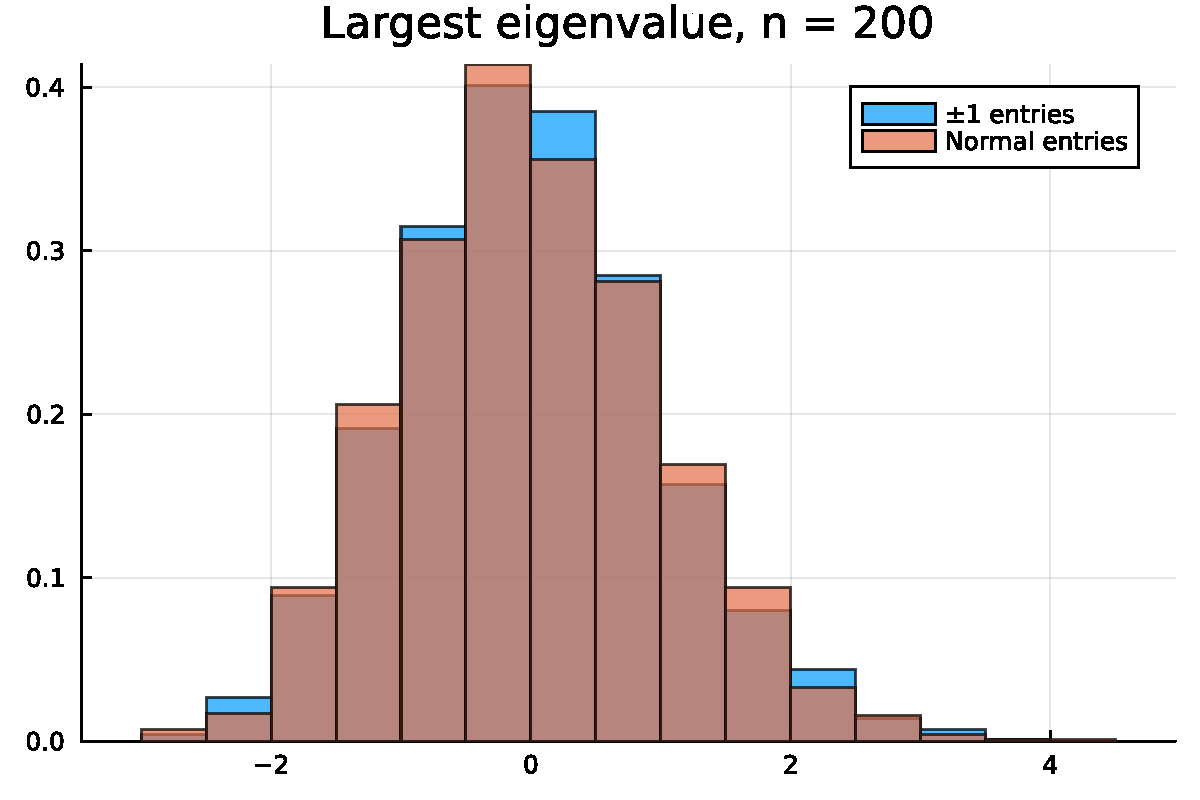
\includegraphics[width=0.6\linewidth,height=0.45\linewidth]{figures/I.Universality_5_1.pdf}

\section{Poster projects}
The possibilities for projects related to universality are endless and I encourage you to think about an original idea. Here are some example projects to help guide you:

\begin{itemize}
\item[1. ] Hermitian random matrices also satisfy universality properties. How do histograms of their eigenvalue statistics (both global and local) compare to the symmetric case?


\item[2. ] A \emph{Wishart ensemble} is a random symmetric matrix $X X^\ensuremath{\top}$ where $X \ensuremath{\in} \ensuremath{\bbR}^{m \ensuremath{\times} n}$ is a rectangular matrix with random entries. It also exhibits universality but depending on the ratio $\ensuremath{\alpha} = m/n$. Can you explore how the global and local statistics behave? Do they match the Wigner ensemble case?


\item[3. ] The spacing of zeros of the Riemann Zeta function on the critical line match the universality. to higher accuracy?


\item[4. ] What happens when the 4-moment condition breaks down? I.e. what are eigenvalue statistics for matrices with heavytailed entries?


\item[5. ] One can consider matrices associated with random networks, a la as discussed in Introduction to Applied Mathematics. How connected does a random network need to be to exhibit universality?

\end{itemize}

